\section{Overview of Quadtree Construction}
\label{app:quadtree}

The first step is to obtain a box enclosing all input points, centered at zero, with all side lengths equal to
$\boxsize$. This can be done as follows: select an arbitrary input point, and translate the dataset so that this point is at the origin. Then, using
$O(nd)$ time, set $\boxsize$ to be the maximum distance from any point to the origin. Having obtained this box, add a random shift $s \leq \boxsize$ is to all the points'
coordinates so that the input is now in the box $[-2\boxsize, 2\boxsize]^d$. This transformation does not change any distances and therefore preserves the
$k$-median cost.  The $i$-th level of the tree (for $i \in \lbra 0, ..., \log \Delta \rbra$) is constructed by centering a grid of side length $2^{-i} \cdot
2\boxsize$ at $0$, making each grid-cell a node in the tree.  The parent of a cell $c$ is simply the cell at level $i-1$ that contains $c$, and the distance
between $c$ and its parent is set to $2^{-i} \cdot 2\boxsize \cdot \sqrt{d}$ (the length of the hypercube's diagonal). This embedding takes $O(nd \log \Delta)$
time to construct, where $\log \Delta$ is the depth of the tree.

\section{Proof of \cref{sec:theory}}\label{app:theory}

We formalize the proof that the \cref{alg:main} produces an $\eps$-coreset in time $\tilde O(nd \log \Delta)$
\begin{proof}
%We show that \cref{alg:main} has the desired guarantees.
First, performing the Johnson-Lindenstrauss embedding takes time $\tilde O(nd)$.

On the projected dataset, the algorithm \fkmeans runs in time $\tilde O\lpar n \log \Delta\rpar$, and the solution it has an approximation-ratio $O\lpar \tilde{d}^z \log k\rpar = O\lpar\log^{z+1} k\rpar$ for $\tilde P$. 
The guarantee offered by the embedding ensure that the clustering $\lbra \calC_1,...,\calC_k\rbra$ still has approximation ratio for $P$ \cite{makarychev2019performance}. 

For $k$-means, computing the $1$-mean solution for each $\calC_i$ takes time $O(nd)$ (the $1$-mean is simply the mean). 
For $k$-median, computing the $1$-median solution can be done as well in time $O(nd)$ \cite{CohenLMPS16}. 
We note that both may be approximated to a factor $2$ in constant time, by sampling uniformly at randm few points from each cluster \cite{neurips21}.

Provided the $c_i$ and the partition $\calC_i$, computing $|\calC_i|$ and $\cost(\calC_i, c_i)$ for all $i$ also takes time $O(nd)$.

Since the solution consisting of assigning each $p \in \calC_i$ to $c_i$ is a $O\lpar \log^{z+1} k\rpar$-approximation, the values $s(p)$ defined in \cref{alg:main} can be used to perform the coreset construction algorithm, and we conclude from \cref{fact:logApprox}.
\end{proof}


\subsection{Reduction to $k$-median.}
\label{app:redKM}

\begin{lemma}
Let $\calS$ be a $c$-approximation for $k$-median on $P$. Then, $\calS$ is a $nc^2$-approximation for $k$-means on $P$.
\end{lemma}
\begin{proof}
Let $\cost_1$ (resp. $\cost_2$) be the $k$-median (resp. $k$-means) cost, $\opt_1$ (resp. $\opt_2$) be the optimal $k$-median (resp. $k$-means) solution. We have the following inequalities:
\begin{align*}
\cost_2(\calS) &= \sum_{p\in P} \dist(p, \calS)^2 \leq \lpar \sum_{p\in P} \dist(p, \calS)\rpar^2\\
&\leq c^2 \cdot \lpar  \sum_{p\in P} \dist(p, \opt_1)\rpar^2\\
&\leq c^2 \cdot \lpar  \sum_{p\in P} \dist(p, \opt_2)\rpar^2\\
&\leq c^2 \cdot n \cdot  \sum_{p\in P} \dist(p, \opt_2)^2,
\end{align*}
where the last inequality stems from Cauchy-Schwarz. Therefore, $\calS$ is a $nc^2$ - approximation to $k$-means. 
\end{proof}


\subsection{Estimation of the Optimal Cost in a Tree}
\label{app:apx-tree-proof}

\begin{proof}[proof of \cref{lem:apxTree}]
If the input is spread in $k+1$ distinct cell at level $i$, then in any solution there is at least one of those cells with no center. In the tree metric, points lying in this cell have therefore connexion cost at least $\sqrt{d}2^{-i+1} \cdot \boxsize$, and thus the left-hand-side of the inequality holds.

On the other hand, if the input is contained into $k$ cells at level $i-1$, then placing arbitrarily a center in each cell yields a solution with cost at most $n \cdot \sqrt{d}2^{-i+4} \cdot \boxsize$: indeed, the distance from any point to its closest center is at most $2 \cdot \sum_{j \geq i-1} \sqrt{d}2^{-j} \cdot 2\boxsize \leq 4 \sqrt{d}2^{-i+2} \cdot \boxsize$ (summing the edge length from the point to the cell at level $i$, and then going down to the center). This concludes.
\end{proof}

\begin{figure*}
\label{fig:lightweight_breaks}
\centering
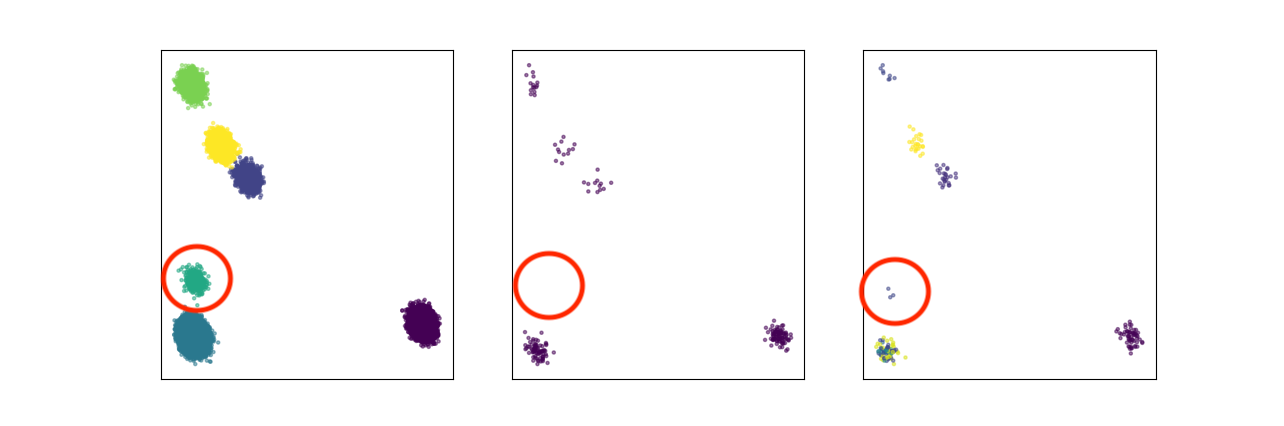
\includegraphics[width=.95\linewidth]{images/lightweight_breaks.png}
\caption{
The results of lightweight and fast-coreset constructions on a dataset of $n=100K$ points with clusters of varying size. Coresets have 200 points.
\emph{Left}: Original multivariate-Gaussian dataset. \emph{Middle}: Lightweight coresets fail to capture the cluster of $\sim$400 points.
\emph{Right}: The Fast-coreset construction runs in linear time but identifies all of the clusters.
}
\end{figure*}

